\chapter{Toma de decisiones}

    Esta sección tratará distintas problemáticas que se han abordado durante el desarrollo del proyecto, de forma que se puedan entender mejor las decisiones tomadas y redactadas en los capítulos anteriores de esta memoria.

    No se incluyen aquellos problemas que se hayan resuelto con investigación, como por ejemplo: saber usar algunas funcionalidades de WordPress, qué casos incluir en los laboratorios, etc.

    \section{Gestión local de contenedores Docker}

        Durante todo el documento se ha hablado de la funcionalidad del proyecto: una plataforma web que permite a los usuarios acceder a laboratorios virtuales donde poner en práctica los conocimientos adquiridos en la propia plataforma, siendo dichos laboratorios contenedores Docker que el usuario puede iniciar o detener a voluntad desde el sitio web, aunque con ciertas limitaciones.
        
        Sin embargo, esto planteaba un problema: cómo se podrían gestionar esos contenedores Docker. 

        \subsection{Conexión entre el sitio web y Docker}

            El objetivo se trataba de algo tan simple como levantar y destruir contenedores Docker, sin embargo, esto debía hacerse de forma dinámica, ya que el resultado final esperado era tener un sistema donde los contenedores no estuvieran permanentemente activos, sino que fueran activados y desactivados en función de su uso.
            
            El uso de estrategias como Kubernetes excedían a las propias necesidades del proyecto, ya que al tratarse de una prueba de concepto no se requería gestionar un gran número de contenedores, ni tampoco era necesario que se organizaran en clústeres; por tanto, se decidió que los contenedores se gestionarían de forma local.

            \begin{figure}[htbp]
                \centering

                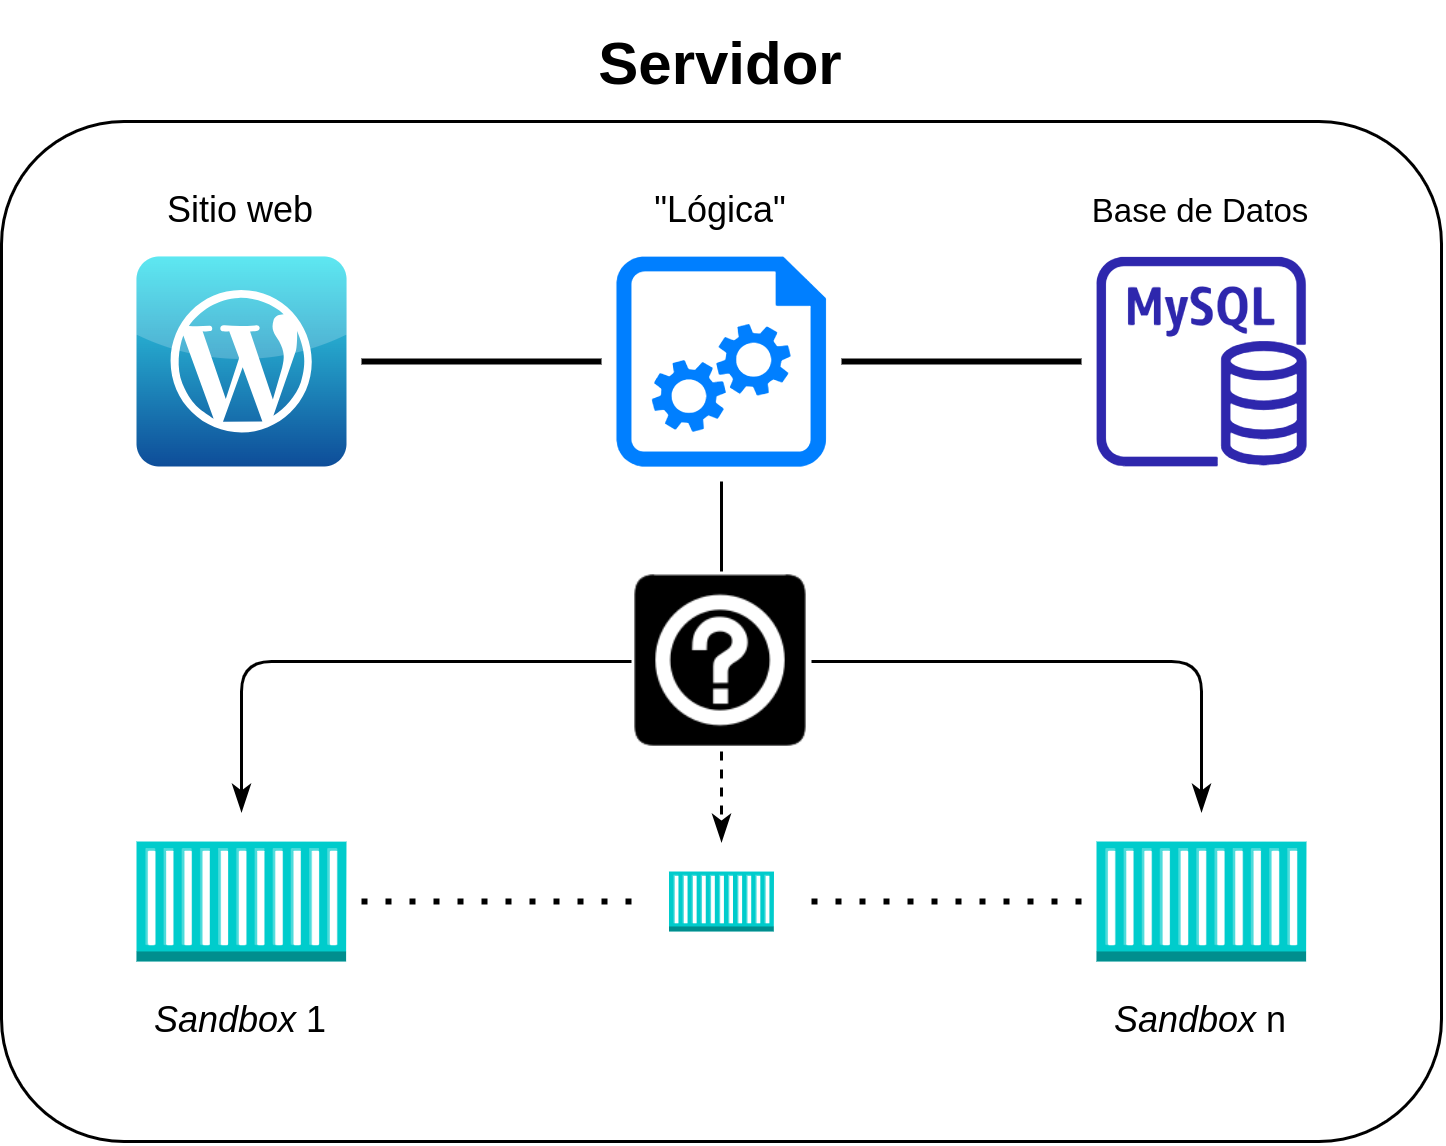
\includegraphics[width=0.5\textwidth]{images/Diagramas/conexion.png}
                \caption{Representación gráfica del problema de conexión entre el sitio y los contenedores}
                \label{fig:conexion}
            \end{figure}

            Tampoco se usaron APIs ni librerías, ya que se consideró que no era necesario, y que se podía hacer uso de los propios comandos del sistema para gestionar los contenedores Docker; de nuevo, porque la idea en sí resultaba muy simple, aunque más tarde su complejidad fue creciendo.

            El resultado final fue el uso del siguiente comando del sistema, que se ejecuta usando \texttt{exec()} en el fichero \texttt{functions.php} del sitio web:
            \\
            
            \begin{lstlisting}[style=php_style]
    exec("docker run --rm -p $puerto/22 -d $laboratorio:latest");
            \end{lstlisting}

            El comando recibe un puerto libre del sistema y el nombre del laboratorio (imagen Docker) para crear el contenedor, indicado como variables PHP en la instrucción anterior. La opción \texttt{--rm} se usa para que el contenedor se destruya automáticamente al detenerse, y la opción \texttt{-d} para que se ejecute en segundo plano (aún en segundo plano devolverá la ID del contenedor creado).


        \subsection{Mapeo de puertos sin solapamientos}

            Por otro lado, se presentaba el siguiente problema, ¿cómo se podría gestionar el mapeo de puertos de los contenedores Docker de forma automática?

            Al no usar Kubernetes, no se podía usar el mapeo de puertos de forma dinámica, ya que los contenedores se gestionaban de forma local y no se podía acceder a ellos desde fuera de la máquina donde se ejecutaban, por lo que se decidió que los contenedores se gestionarían de forma local.

            \begin{figure}[htbp]
                \centering

                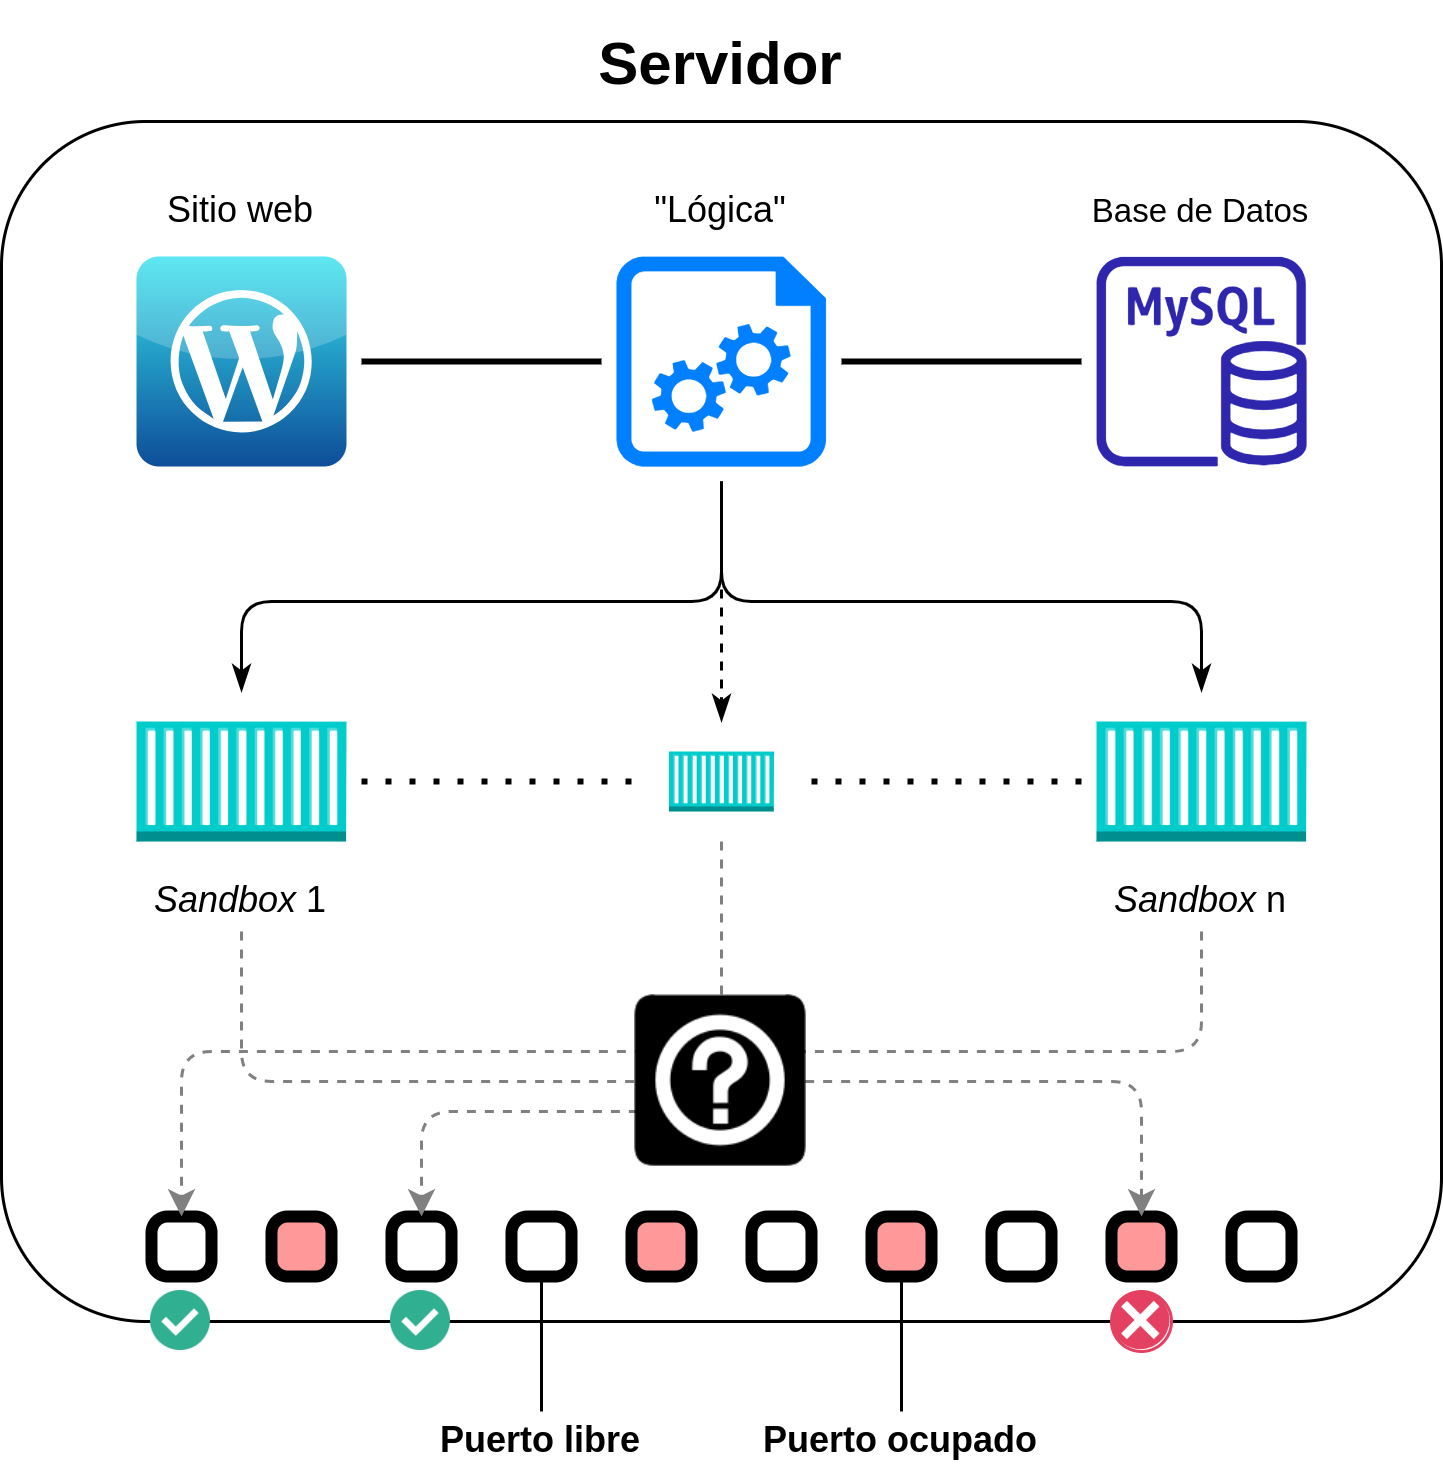
\includegraphics[width=0.5\textwidth]{images/Diagramas/puertos.png}
                \caption{Representación gráfica del problema de mapeo de puertos}
                \label{fig:mapeo-puertos}
            \end{figure}

            La opción \texttt{-p} de Docker permite mapear puertos de forma estática, lo que implica que si se usaba un puerto que ya estuviera en uso, la creación del contenedor fallaría.
            
            Por otra parte, es posible usar un rango de puertos con esa opción, lo que permite a Docker mapear un puerto del contenedor a cualquier puerto libre en el rango específicado de forma automática y aleatoria (la selección no es secuencial); esta parecería la opción perfecta pero tenía una gran limitación: los puertos libres de un rango de puertos solo son conocidos entre los contenedores de la misma imagen, y por tanto, como cada laboratorio es una imagen Docker de la que se construyen contenedores para los usuarios, esto quiere decir que no era posible determinar todos los puertos libres para todas las imágenes.
            
            Otra opción que se contempló fue la de usar el mismo rango para todas las imágenes, pero uno tan amplio que se redujera todo lo posible la posibilidad de colisiones de puertos entre contenedores de distintas imágenes; sin embargo, esta opción fue descartada porque, aunque pudiera haber sido efectiva en esta prueba de concepto, no dejaba de existir la posibilidad de que se produjeran colisiones, y por tanto, no se consideró una solución aceptable.

            El uso de ficheros \texttt{docker-compose.yml} también era muy restrictivo, ya que no permitía la gestión dinámica de puertos; para ser más específicos, este fichero almacena una configuración a la que se puede llegar usando combinaciones de opciones y valores de comandos Docker, por lo que no añade ninguna funcionalidad adicional, sino que solo permite almacenar una configuración. Aquí se reptite exactamente el mismo problema de las colisiones descrito en el párrafo anterior.

            Finalmente, se optó por generar puertos disponibles usando código en \texttt{functions.php}: se define un rango inicial \texttt{(5555 - 9999)} predefinido y para cada laboratorio que quiere iniciar un usuario, se busca en la base de datos qué puertos están siendo ocupados por otros laboratorios, se calcula la diferencia entre el rango inicial y los puertos ocupados, y se selecciona un puerto aleatorio dentro de ese rango.

            Como el puerto obtenido se usa para el laboratorio, al almacenarse esa información en la base de datos, el puerto queda registrado; del mismo modo cuando el usuario o la tarea de cron destruyan un laboratorio, los datos serán liberados de la base de datos y el puerto volverá a estar disponible para su uso.


    \section{Limitaciones del uso de contenedores y Docker}
        
        Cuando una persona piensa en la ciberseguridad, se imagina la clásica imagen de un hacker tecleando comandos en una pantalla llena de terminales, pero lo cierto es que aunque muchas herramientas se usan como scripts o comandos, no todas son así y algunas requieren una interfaz gráfica para su uso.

        Sin embargo, ocurre que para este caso concreto, no podrían usarse contenedores para aplicaciones que se usen con GUI. Los contenedores pueden llegar a ejecutar aplicaciones gráficas, pero esto implicaría que los usuarios descargaran la imagen y ellos crearan los contenedores, porque si no, estarían abriendo la aplicación en el servidor, donde no tienen acceso más allá de del acceso al contenedor por SSH.

        En algunas ocasiones es posible ejecutar una GUI a través del navegador, lo que sumado al mapeo de puertos, podría permitir que el usuario accediera a la aplicación, pero esto no es posible en todos los casos y además, no es una solución que se pueda aplicar de forma genérica.
        
        Por otra parte, existe la limitación actual de solo abrir y mapear un puerto por contenedor, teniendo que tomar la decisión sobre qué hacer en cada caso o qué finalidad tiene el laboratorio: entorno virtualizado con herramientas preinstaladas y casos de uso para dichas herramientas, o contenedor vulnerable con el que trabajar desde una máquina virtual propia del usuario.


    \section{Procesos bajo el usuario \texttt{www-data}}

        Al no usar una herramienta externa como Kubernetes, todos los procesos se realizan de forma local, por lo que el usuario que ejecuta los comandos es el usuario que ejecuta el servidor web, en este caso, \texttt{www-data}.

        Esto quiere decir que para que el proyecto funcione, el usuario \texttt{www-data} debe ser el que inicie el servicio de Docker, por lo que debe tener permisos para ello.
        \\

        \begin{lstlisting}[style=bash_style]
    $ sudo -u www-data systemctl start docker            
        \end{lstlisting}

        \begin{lstlisting}[style=comment_style]
    sudo: ejecutar un comando como otro usuario.
        -u: especificar el usuario.
    systemctl: gestionar servicios del sistema.
        \end{lstlisting}

        Por otra parte, también necesario añadir el usuario \texttt{www-data} al grupo \texttt{docker} para que pueda ejecutar los comandos de Docker.
        \\

     \begin{lstlisting}[style=bash_style]
    $ sudo usermod -aG docker www-data
        \end{lstlisting}

        \begin{lstlisting}[style=comment_style]
    sudo: ejecutar un comando como otro usuario.
    usermod: modificar un usuario.
        -aG: a&ñ&adir (a) a un grupo (G).
        \end{lstlisting}

        Una vez añadido, puede comprobarse que el usuario \texttt{www-data} pertenece al grupo \texttt{docker} usando el comando \texttt{groups} o el comando \texttt{id}.
        \\

        \begin{lstlisting}[style=bash_style]
    $ groups www-data

    www-data : www-data docker
        \end{lstlisting}

        \begin{lstlisting}[style=comment_style]
    groups: mostrar los grupos a los que pertenece un usuario.

    Este comando solo muestra los grupos a los que pertenece el usuario indicado.
        \end{lstlisting}

        \begin{lstlisting}[style=bash_style, basicstyle=\ttfamily\scriptsize]
    $ id www-data

    uid=33(www-data) gid=33(www-data) groups=33(www-data),999(docker)
        \end{lstlisting}

        \begin{lstlisting}[style=comment_style]
    id: mostrar informaci&ó&n sobre un usuario.

    Este comando muestra diversas caracter&í&sticas del usuario:
        uid: identificador de usuario en el sistema.
        gid: identificador de grupo de usuario en el sistema.
        groups: identificadores de grupos del usuario.
        \end{lstlisting}

        Además, del mismo modo, tendrá que crear previamente todas las imágenes de los laboratorios para que aparezcan disponibles en Docker y pueda utilizarlas: las imágenes Docker creadas por un usuario solo son visibles para ese usuario, por lo que si el usuario \texttt{www-data} no crea las imágenes, no podrá usarlas.

        Durante el desarrollo del proyecto se creó un repositorio para la creación de los laboratorios y se incluyó un script con el que actualizar las imágenes de laboratorios en el servidor, así como añadir laboratorios que no estuvieran previamente. Este script automatiza el proceso de creación de imágenes, por lo que puede ejecutarse del mismo modo que se ha mostrado con las capturas anteriores.
        \\

        \begin{lstlisting}[style=bash_style]
    $ sudo -u www-data ./instalar.sh

    Imagen: 01_intro-linux
        Duplicada.
        Actualizando...
        Actualizada.

    Imagen: 02_intro-bash
        Duplicada.
        Actualizando...
        Actualizada.

    Imagen: 03_intro-redes
        Creando...
        Creada.

    Imagen: (...)

    Laboratorios creados:
    * 01_intro-linux
    * 02_intro-bash
    * 03_intro-redes
    * (...)
        \end{lstlisting}

        Y por último, pasa lo mismo con la tarea de cron que automatiza la destrucción de los laboratorios: debe ser el usuario \texttt{www-data} quien defina y active la tarea de cron.
        \\

        \begin{lstlisting}[style=bash_style]
    $ sudo -u www-data crontab -e
        \end{lstlisting}

        \begin{lstlisting}[style=comment_style]
    El comando sudo permite ejecutar un comando como otro usuario, en este caso, www-data.

    El comando crontab permite gestionar las tareas de cron, en este caso, se edita la tarea de cron del usuario www-data.
        \end{lstlisting}

        La tarea de cron defindia es la siguiente:
        \\

        \begin{lstlisting}[style=bash_style, caption={contenido del fichero},captionpos=b, basicstyle=\ttfamily\scriptsize]
    # To define the time you can provide concrete values for
    # minute (m), hour (h), day of month (dom), month (mon),
    # and day of week (dow) or use '*' in these fields (for 'any').
    # 
    # For more information see the manual pages of crontab(5) and cron(8)
    # 
    # m h  dom mon dow   command

    * * * * * /bin/bash /var/www/html/scripts/stop-1h-container.sh > /var/www/html/scripts/stop-1h-container.log 2>&1
        \end{lstlisting}

        \cleardoublepage



\chapter{Manual de usuario}

    \section{Plataforma}

        Esta sección depende en su mayoría de la experiencia del usuario con WordPress; no obstante, se incluyen instrucciones para las funcionalidades más importantes y relacionadas con la elaboración del proyecto.

        Se debe asumir que todo lo establecido en esta sección hace referencia sola y exclusivamente a la plataforma web y su contenido.

        \subsection{Anotaciones previas}

            \subsubsection{Copia de seguridad con WPvivid}

                WPvivid \cite{wpvivid} es un plugin de WordPress que permite realizar copias de seguridad de un sitio web, así como restaurarlas; WordPress funciona almacenando toda su configuración y contenido en una base de datos, por lo que el plugin se encarga, ensencialmente, de hacer una copia de la base de datos y de los ficheros de la plataforma en formato \texttt{.zip}.

                Existe un fichero de copia de seguridad de la plataforma hecha con WPvivid. Esta se puede usar tanto para restaurar los datos de la plataforma, como para duplicarla en otro sitio web de WordPress; para esta segunda opción, se recomienda seguir los siguientes pasos:
                
                \begin{enumerate}
                    \item Crear un nuevo sitio web de WordPress.
                    \item Instalar el plugin WPvivid.
                    \item Importar la copia de seguridad.
                    \item Restaurar la copia de seguridad.
                \end{enumerate}

                \begin{figure}
                    \centering

                    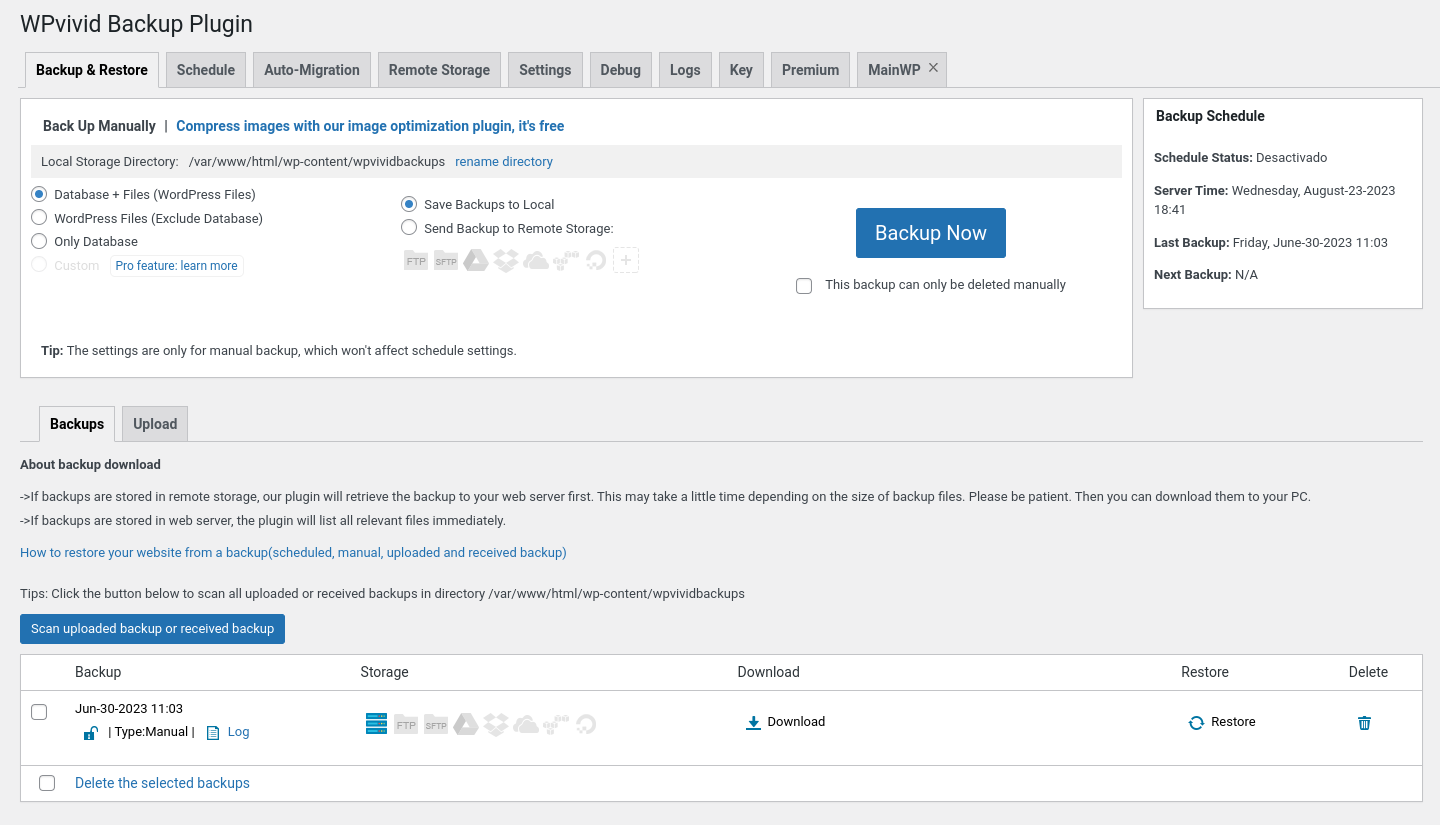
\includegraphics[width=0.75\textwidth]{images/Capturas/localhost/wpvivid.png}
                    \caption{Gestión de copias de seguridad con WPvivid}
                    \label{fig:wpvivid}
                \end{figure}

                Esto convertirá cualquier sitio web de WordPress vacío en una copia exacta del sitio web de la plataforma actual.
                
                \paragraph{Importante}
                
                    Cabe destacar que, como se mencionó anteriormente, se copiará toda una base de datos, sobreescribiendo toda la información del sitio original, incluyendo las credenciales de los usuarios y administradores; por ello, la entrega también incluye una copia de las credenciales de un usuario administrador que se aconseja encarecidamente modificar una vez se haya importado la copia de seguridad.

        \subsection{Añadir un laboratorio}

            WordPress permite la creación de contenido personalizado, más allá de sus tipos predefinidos (Páginas, Entradas, etc.), por ello se ha creado un tipo de contenido personalizado llamado \textit{Laboratorios}, disponible desde el menú lateral.

            \begin{figure}[!htbp]
                \centering

                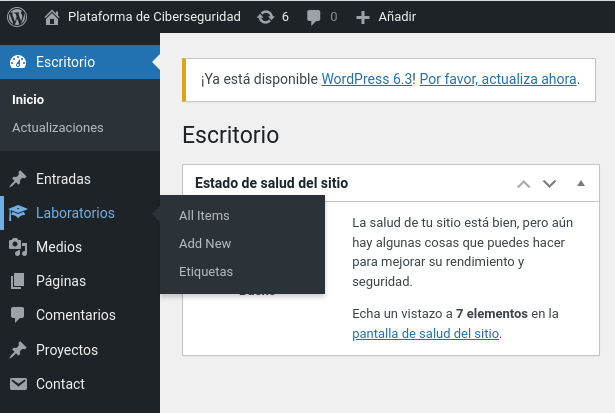
\includegraphics[width=0.75\textwidth]{images/Capturas/localhost/laboratorios.png}
                \caption{Menú de laboratorios}
                \label{fig:laboratorios}
            \end{figure}

            Una vez dentro, se puede crear un nuevo laboratorio usando el botón \textit{Añadir nuevo} en la parte superior o usando el desplegable anterior.

            Un laboratorio solo consta de 2 elementos: un texto descriptivo del concepto que se está tratando, que puede estar escrito en Markdown o HTML (recomendable este último); un identificador de un laboratorio, en la parte inferior, que no es más que \textbf{el nombre de la imagen Docker del sistema} que corresponde al laboratorio.

            \begin{figure}[!htbp]
                \centering

                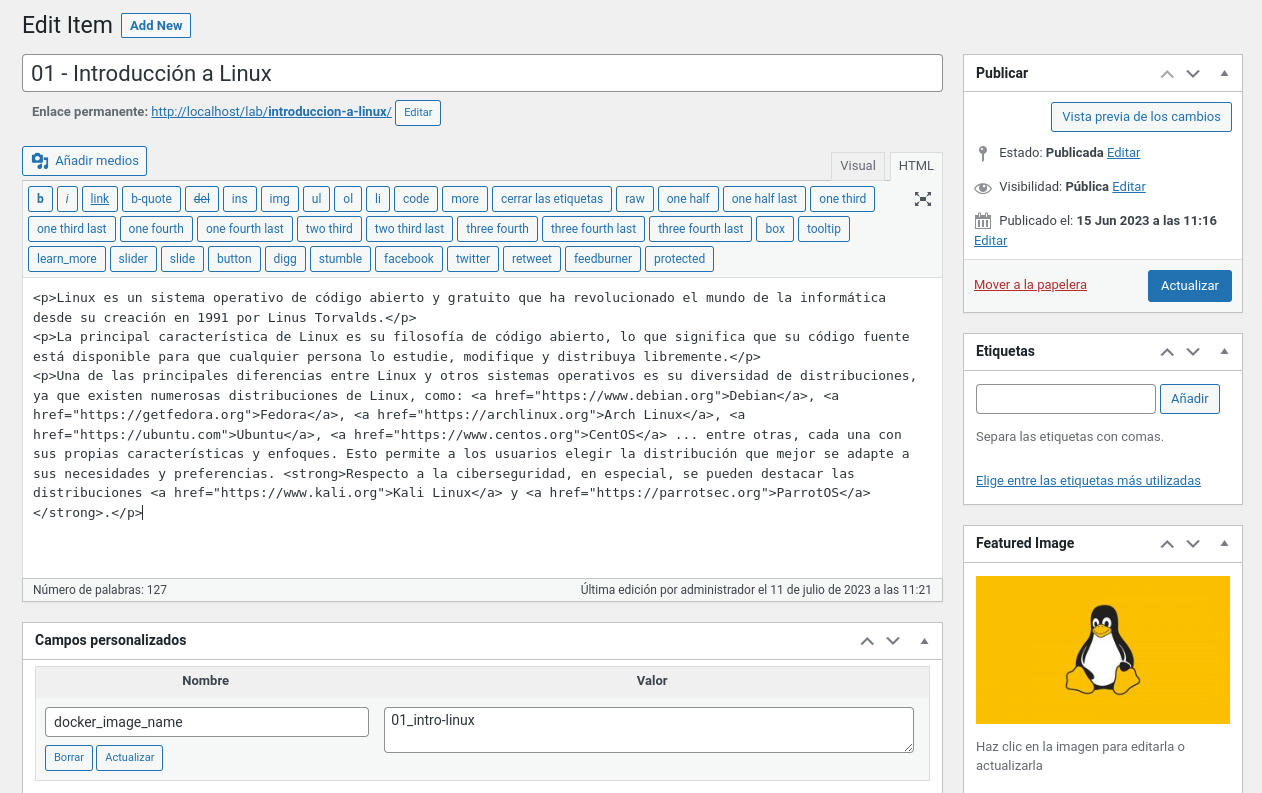
\includegraphics[width=0.75\textwidth]{images/Capturas/localhost/creacion.png}
                \caption{Creación de un laboratorio}
                \label{fig:anadir-laboratorio}
            \end{figure}

            También es posible añadir opcionalmente una imagen de cabecera que se mostrará en la lista de laboratorios disponibles. Esta imagen debe ser local y una vez publicada en el sitio, formará parte de los archivos locales del mismo.

            \paragraph{Nota}
            
                Consulte la sección \ref{sec:construir-laboratorio} para saber más sobre la gestión de los laboratorios.

        \subsection{Modificar o eliminar un laboratorio}

            Cualquier laboratorio se puede modificar desde la lista de laboratorios disponibles, accediendo a la opción \textit{Laboratorios} del menú lateral.

            Modificar o eliminar un laboratorio consiste exclusivamente en el uso de las opciones de edición de contenido de WordPress, por lo que no se requieren instrucciones adicionales.

            Sin embargo, se debe tener en cuenta que esta modificación solo afecta al contenido de la plataforma, por lo que si se desea aplicar alguna modificación al laboratorio en sí, será necesario modificar la imagen Docker correspondiente.

            \paragraph{Nota}

                Si se modifica el nombre de la imagen Docker o esta se elimina, recuerde que también debe modificar el atributo \texttt{docker\_image\_name} del \textit{Laboratorio} de WordPress.

            \newpage


    \section{Laboratorios}

        Los laboratorios se han llevado a cabo en un repositorio distinto y será necesario un \textit{clon} del mismo en el sistema para que la plataforma pueda referenciarlos.

        La conexión que se establece entre la plataforma y los laboratorios virtualizados es la siguiente: \textbf{la plataforma solo se encarga de crear y destruir contenedores Docker, por lo que los laboratorios son imágenes Docker en el servidor donde se aloja la plataforma}.

        Esto quiere decir que será necesario previamente construir las imágenes de los laboratorios en el servidor, para que la plataforma pueda usarlas.

        \paragraph{Nota}

            Como es la plataforma la que construye y destruye los laboratorios a petición de sus usuarios, todos los comandos de Docker de esta sección se deben ejecutar como el usuario \texttt{www-data}, ya que es el usuario que ejecuta el servidor web y por tanto, el que ejecuta los comandos de Docker.

        \subsection{Construir los laboratorios originales}

            Si se quiere usar los laboratorios originales, la forma más eficaz es ejecutar el script de instalación como se describe en la sección \ref{sec:construir-laboratorio}.

        \subsection{Definir un laboratorio nuevo}

            Se entiende como \textit{laboratorio} a una carpeta dentro de \texttt{labs/} cuyo contenido es, como mínimo, los siguientes ficheros:
            
            \begin{itemize}
                \item \texttt{Dockerfile}: instrucciones para crear la imagen Docker del laboratorio.
                \item \texttt{README.html}: descripción del laboratorio en formato HTML.
            \end{itemize}

            Por tanto, crear un laboratorio es tan sencillo como crear un fichero \texttt{README.html} que explique el concepto a tratar (teoría) y un fichero \texttt{Dockerfile} que contenga las instrucciones para crear la imagen Docker del que extraer posteriormente los contenedores (práctica).

            Adicionalmente, algunos laboratorios también cuentan con una carpeta \texttt{resources/} que contiene recursos necesarios para la construcción de la imagen Docker.

            \paragraph{Nota}
                
                Cabe destacar que todos los ficheros descriptivos \texttt{README.html} han sido generados a partir de un fichero más simple: \texttt{README.md}, escrito en Markdown. Este archivo, pese a no ser necesario, está incluido en todos los laboratorios del repositorio; esto se debe a que el repositorio está publicado en GitHub y al llamarse estrictamente \textit{README.md}, su contenido se procesa y se muestra en la web, lo que permite una mejor visualización del contenido del laboratorio.

        \subsection{Construir un laboratorio nuevo}
            \label{sec:construir-laboratorio}

            Una vez se ha definido un laboratorio, existen 2 alternativas para construir el laboratorio:

            \subsubsection{Docker}

                Usando el comando de Docker para construir imágenes Docker:
                \\

                \begin{lstlisting}[style=bash_style]
    $ sudo -u www-data docker build {ruta} -t {nombre}
                \end{lstlisting}

                \begin{lstlisting}[style=comment_style]
    sudo: ejecutar un comando como otro usuario.
        -u: especificar el usuario.
    docker: comando para gestionar Docker.
        build: subcomando para construir una imagen Docker.
            -t: etiqueta (nombre) para la imagen Docker.
                \end{lstlisting}

                \paragraph{Nota}

                    El nombre de la imagen Docker será la que se use en el atributo \texttt{docker\_image\_name} del \textit{Laboratorio} de WordPress.

            \subsubsection{Script de instalación}

                El repositorio incluye un script de instalación que permite tanto construir por primera vez nuevos laboratorios, como actualizar aquellos que hayan sido modificados.

                Este script es \texttt{/labs/instalar.sh} y se debe ejecutar desde su ubicación:
                \\

                \begin{lstlisting}[style=bash_style]
    $ cd labs/
    $ chmod +x instalar.sh
    $ ./instalar.sh
                \end{lstlisting}

                \begin{lstlisting}[style=comment_style]
    cd: cambiar de directorio.
    chmod: modificar los permisos de un fichero.
        +x: a&ñ&adir permisos de ejecucion.

    instalar.sh: crea o actualiza cada laboratorio de labs/.
        Si existe una imagen con el mismo nombre, se actualiza;
        en caso contrario, se crea una nueva imagen Docker.
                \end{lstlisting}

                Una vez llevado cualquiera de ambos procesos, el laboratorio estará disponible para su uso en la plataforma, ya que pertenecería a la lista de imágenes de Docker.

                Se puede comprobar el funcionamiento correcto de ambas formas con el comando:
                \\

                \begin{lstlisting}[style=bash_style]
    $ sudo -u www-data docker images
                \end{lstlisting}

                \begin{lstlisting}[style=comment_style]
    sudo: ejecutar un comando como otro usuario.
    docker: comando para gestionar Docker.
        images: subcomando para listar las imagenes Docker.
                \end{lstlisting}

                \paragraph{Nota}

                    El nombre de la imagen Docker será la que se use en el atributo \texttt{docker\_image\_name} del \textit{Laboratorio} de WordPress.

        \subsection{Modificar o eliminar un laboratorio}

            Cualquier laboratorio se puede modificar a partir de su carpeta correspondiente, modificando su \texttt{Dockerfile}. Una vez se ha modificado, se debe reconstruir la imagen Docker del laboratorio para que los cambios surtan efecto, aplicando cualquier de las opciones descritas en la sección anterior.

            \paragraph{Nota}

                Recuerde modificar el atributo \texttt{docker\_image\_name} del \textit{Laboratorio} de WordPress si se modifica el nombre de la imagen Docker o esta se elimina.

                \cleardoublepage

            

\chapter{Código desarrollado}

    \section{Scripts para la plataforma}

        \subsection{Gestión del tiempo de vida de contenedores}
            
            \begin{lstlisting}[style=bash_style, basicstyle=\ttfamily\scriptsize]
    #!/bin/bash


    # Variables "globales"
    CONTENEDORES=$(docker ps -q)    # Lista de contenedores activos (IDs)
    VIDA=3600                       # Tiempo de vida de un contenedor (en segundos)


    # Mostrar informacion de la ejecucion
    echo -e "\e[1mEjecucion actual: $(date +%H:%M:%S)\e[0m\n"
    if [ -z "$CONTENEDORES" ]; then
        echo -e "No hay contenedores activos.\n"
    else
        echo -e "Hay $(echo $CONTENEDORES | wc -w) contenedores activos.\n"
    fi


    # Recorrer los contenedores activos
    for CONTENEDOR in $CONTENEDORES; do
        # Tiempo de creacion del contenedor (ISO 8601)
        CREACION=$(docker inspect --format '{{ .State.StartedAt }}' $CONTENEDOR)

        INICIO=$(date --date="$CREACION" +%s)       # Tiempo de ejecucion (en segundos)
        AHORA=$(date +%s)                           # Tiempo actual (en segundos)
        DIFF=$(( $AHORA - $INICIO ))                # Tiempo transcurrido (en segundos)

        # Crear informacion del estado de un contenedor
        MSG="$CONTENEDOR:\t$DIFF / $VIDA segundos."

        # Comprobar que el contenedor supero el tiempo de vida
        if [ $DIFF -gt $VIDA ]; then
            echo -e "$MSG \e[31mTiempo de vida alcanzado.\e[0m"
            
            docker stop $CONTENEDOR > /dev/null

        else
            if [ $DIFF -gt $(( $VIDA - 60 )) ]; then
                echo -e "$MSG \e[33mDestruccion inminente.\e[0m"
            else
                echo -e "$MSG \e[32mDisponible.\e[0m"
            fi
        fi
    done

    echo
            \end{lstlisting}
    
            \newpage

            Con el fin de optimizar los recursos, la plataforma no tendrá laboratorios activos cuando esta no se esté usando, por lo que se ha creado una tarea de cron que se ejecuta cada minuto y comprueba si hay contenedores activos, y en caso de haberlos, comprueba si alguno ha superado el tiempo de vida establecido (1 hora por defecto) y lo destruye.

            El script anterior se encarga de comprobar el tiempo que el contenedor de un laboratorio ha estado activo, y lo destruye cuando este supera el tiempo establecido.
        
            El script realiza las siguientes acciones:

            \paragraph{Obtener los contenedores activos}
            
                Usando el comando \texttt{docker ps -q} se obtiene una lista de los contenedores activos, pero solo sus IDs, lo que permite recorrerlos de forma más sencilla; esta información se almacena en la variable \texttt{CONTENEDORES}, que se usará para recorrer los contenedores activos.

            Para cada contenedor de la lista anterior, se realizan los siguientes procesos:

            \paragraph{Obtener el tiempo de creación}
            
                Usando el comando \texttt{docker inspect --format '\{\{ .State.StartedAt \}\}'} se obtiene el tiempo de creación de un contenedor en formato ISO 8601, que es el formato que usa Docker para almacenar la fecha y hora de creación de un contenedor; esta información se almacena en la variable \texttt{CREACION}.

            \paragraph{Obtener el tiempo de ejecución}
            
                Usando el comando \verb|date --date="$CREACION" +%s| se obtiene el tiempo de ejecución de un contenedor en segundos, y usando el comando \verb|date +%s| se obtiene el tiempo actual en segundos; con estos dos valores se calcula la diferencia entre ellos, que es el tiempo que ha estado activo el contenedor; esta información se almacena en la variable \texttt{DIFF} y corresponde a los segundos que han pasado desde que se creó el contenedor hasta el momento actual.

            \paragraph{Comprobar si el contenedor debe detenerse}

                Finalmente, se comprueba si el contenedor ha superado el tiempo de vida establecido, y en caso de haberlo superado, se detiene el contenedor usando el comando \texttt{docker stop \$CONTENEDOR}.

                Cabe destacar que el script muestra la información correspondiente por la pantalla, pero la tarea cron redirige su salida a \texttt{/dev/null}, por lo que no se mostrará nada por pantalla cuando se ejecute la tarea de cron; sin embargo, el script puede ejecutarse manualmente y observar el estado de los contenedores en cualquier momento.

                \newpage

        \subsection{Actualización de los laboratorios}
        
            \begin{lstlisting}[style=bash_style, basicstyle=\ttfamily\scriptsize]
    #!/bin/sh


    # Variables
    carpetas=$(ls -d */ | grep -v '^logs/$' | sed 's#/##')  # Carpetas del repositorio
    log=logs/$(date +"%Y-%m-%d %H-%M").log                  # Archivos de registro
    duplicada=false                                         # Imagenes duplicadas


    # Crear la carpeta de registros
    mkdir -p logs                       # Si ya existe 'logs' no hace nada


    # Construccion de las imagenes
    for carpeta in $carpetas; do

        echo "$carpeta\n------------------------------------------------" >> $log

        echo "Imagen: $carpeta"


        # Comprobar que la carpeta tiene un Dockerfile
        if [ ! -f $carpeta/Dockerfile ]; then
            echo "    No tiene Dockerfile.\n"
            continue
        fi
    
    
        # Eliminar la version anterior de la imagen
        if [ ! -z "$(docker images -q $carpeta)" ]; then
            duplicada=true
            docker rmi $carpeta >> $log 2>&1
        fi


        # Construir la imagen actual
        if [ ! $duplicada = true ]; then
            echo "    Construyendo..."
        else
            echo "    Actualizando..."
        fi

        docker build -t $carpeta $carpeta/ >> $log 2>&1


        # Almacenar la imagen en una lista si se creo correctamente
        if [ ! -z "$(docker images -q $carpeta)" ]; then
            if [ ! $duplicada = true ]; then
                echo "    Creada.\n"
            else
                echo "    Actualizada.\n"
            fi

            images="$images $carpeta"
        fi

        echo "\n" >> $log

        duplicada=false
    done


    # Mostrar todas las nuevas imagenes generadas
    echo "Resumen:"

    for image in $images; do
        echo "* $image"
    done                
            \end{lstlisting}

            \newpage

            Los entornos virtualizados de la plataforma están compuestos por imágenes Docker, que son creadas a partir de un fichero \texttt{Dockerfile} que contiene las instrucciones necesarias para crear la imagen. Estas imágenes son los laboratorios, y siguiendo la misma estructura planteada en el repositorio de laboratorios, es posible tanto añadir, modificar o eliminar más contenedores a la plataforma.

            Técnicamente, no es necesario que los laboratorios pertenezcan al repositorios, lo esencial es que su imagen Docker esté construida en el sistema y disponible para el usuario \texttt{www-data}. Sin embargo, el repositorio permite gestionar los laboratorios de forma más sencilla, ya que solo es necesario añadir una carpeta con el nombre del laboratorio y el fichero \texttt{Dockerfile} dentro.

            El script anterior contenido en la carpeta \texttt{labs/} del repositorio, y permite hacer un barrido del mismo y crear aquellos laboratorios que no estén presentes en el sistema, así como actualizar aquellos que hayan sido modificados.
            
            El script realiza las siguientes acciones:

            \paragraph{Obtener las carpetas del repositorio}
            
                Usando el comando \verb|ls -d */| se obtienen todas las carpetas del repositorio, y usando el comando \verb|grep -v '^logs/$'| se filtran todas las carpetas excepto la carpeta \texttt{logs/}, que es donde se almacenan los registros de las ejecuciones del script; finalmente, usando el comando \verb|sed 's#/##'| se elimina el carácter \texttt{/} de cada carpeta, ya que no es necesario para el script. Esto resulta en una lista de nombres que se usarán para crear las imágenes Docker.

            \paragraph{Crear la carpeta de registros}

                Usando el comando \texttt{mkdir -p logs} se crea la carpeta \texttt{logs/} en caso de que no exista, y en caso de existir, no hace nada. Esto hace que se puedan comprobar los registros de ejecuciones anteriores y los fallos en la construcción de las imágenes Docker de los laboratorios.

            Acto seguido, para cada carpeta de la lista obtenida al inicio, se realizan los siguientes procesos:

            \paragraph{Eliminar la imagen anterior}

                Usando el comando \verb|docker images -q $carpeta| se comprueba si existe una imagen con el nombre de la carpeta actual, y en caso de existir, se elimina usando el comando \verb|docker rmi $carpeta|; esto produce que se actualice una imagen existente. La imagen se elimina previamente debido a que si se crea una imagen con el mismo nombre que otra, Docker no elimina la anterior, sino que la renombra a \texttt{<none>}.

            \paragraph{Construir una imagen}

                Usando el comando \texttt{docker build -t \$carpeta \$carpeta/} se construye la nueva imagen Docker usando el fichero \texttt{Dockerfile} de la carpeta actual, y se le asigna el nombre de dicha carpeta; esto permite que la imagen tenga el mismo nombre que la carpeta, y por tanto, que sea más fácil de identificar.

            \paragraph{Almacenar la imagen en una lista}

                Usando el comando \verb|docker images -q $carpeta| se comprueba si existe una imagen con el nombre de la carpeta actual, lo que indicaría que la imagen se creó correctamente, y en caso de existir, se añade el nombre de la carpeta a la variable \texttt{images}, que se usará para mostrar las imágenes creadas al finalizar la ejecución del script.

            Finalmente, se muestran las imágenes creadas en la ejecución del script.

        \subsection{Instalación de Kali Linux usando Vagrant}

            \begin{lstlisting}[style=bash_style, basicstyle=\ttfamily\scriptsize]
        #!/bin/bash


        VF_DIR="$HOME/Vagrant/Kali"     # Ubicacion por defecto


        # Actualiza la ubicacion por defecto para el Vagrantfile.
        # Argumentos:
        #   $1: Nueva ruta del Vagrantfile
        function define_directory {
            # Se recibe un argumento y es valido
            if [[ $# -eq 1 && -n "$1" ]]; then
                VF_DIR="$1"
            fi

            echo "Ubicacion del Vagrantfile: $VF_DIR"
        }

        # Instala las dependencias necesarias para la maquina
        # virtual, que en este caso son: Vagrant y VirtualBox.
        function install_dependencies {
            echo "Instalando dependencias..."

            sudo apt-get update -qq
            sudo apt-get install -y vagrant virtualbox > /dev/null 2>&1

            # Comprobar si se han instalado correctamente
            if [[ $? -eq 0 ]]; then
                echo "Paquetes instalados correctamente."
            else
                echo "Error al instalar los paquetes."
                exit 1
            fi
        }

        # Crea el directorio para el Vagrantfile.
        function build_directory {
            # Directorio para los archivos de Vagrant
            if [[ -d $VF_DIR && -f $VF_DIR/Vagrantfile ]]; then
                echo "El directorio seleccionado no esta vacio."
                read -p "Sobreescribirlo? [s/n]: " answer

                # Comprobar si debe reemplazarse
                if [[ "$answer" != "${answer#[Ss]}" ]]; then
                    echo "Reiniciciando el directorio '$VF_DIR'..."
                    rm -rf $VF_DIR
                else
                    echo "No se puede continuar."
                    exit 1
                fi
            else
                echo "Creando el directorio '$VF_DIR'..."
            fi

            mkdir -p $VF_DIR

            # Comprobar si se han creado correctamente
            if [[ $? -eq 0 ]]; then
                echo "Directorio creado correctamente."
            else
                echo "Error al crear el directorio."
                exit 1
            fi
        }

        # Crea la maquina virtual de Kali Linux usando Vagrant.
        function build_kali {
            cd $VF_DIR

            echo "Creando la maquina virtual de Kali Linux..."
            vagrant init elrey741/kali-linux_amd64  > /dev/null     # Inicializar Vagrant
            vagrant up                                              # Inicializar la MV
        }


        # Inicio del script
        install_dependencies    # Instalar las dependencias
        define_directory $1     # Actualizar la ubicacion de la MV
        build_directory         # Crear el directorio
        build_kali              # Crear la MV de Kali Linux

        echo "Fin de la instalacion."
            \end{lstlisting}

            La plataforma también ofrece a los usuarios una forma de instalar una máquina virtual de Kali Linux usando una herramienta llamada Vagrant, que permite crear y gestionar máquinas virtuales de forma sencilla.

            El script anterior permite realizar la instalación desde cero, instalando Vagrant y VirtualBox, creando un directorio para la máquina virtual y creando la máquina virtual de Kali Linux usando Vagrant.

            Este script se trata de una herramienta de desarrollo para agilizar la ejecución de pruebas; la plataforma ya cuenta con un apartado donde se describen estos mismos pasos, con comandos, para que el usuario pueda replicarlo.

            El script realiza las siguientes acciones:

            \paragraph{Instalar las dependencias}

                Usando la función \texttt{install\_dependencies} se instalan las dependencias necesarias para la máquina virtual, que en este caso son Vagrant y VirtualBox.

                Usando el comando \texttt{apt-get update -qq} se actualiza la lista de paquetes disponibles en el sistema sin mostrar información por pantalla, y usando el comando \texttt{apt-get install -y vagrant virtualbox} se instalan los paquetes \texttt{vagrant} y \texttt{virtualbox}, enviando la salida a \texttt{/dev/null} para que no se muestre información por pantalla.

                Además, se comprueba si la instalación se ha realizado correctamente usando el código de salida del comando anterior, que es 0 si se ha realizado correctamente, y 1 si ha habido algún error; en caso de error, el script se detiene.

            \paragraph{Definir la ubicación del Vagrantfile}
            
                Usando la función \texttt{define\_directory} actualiza la ubicación del Vagrantfile por la ruta recibida como argumento \texttt{\$1} del script; si no se recibe ninguna ruta, se usa la ruta por defecto \texttt{\$HOME/Vagrant/Kali}.

            \paragraph{Crear el directorio}

                Usando la función \texttt{build\_directory} se crea el directorio donde se almacenará el Vagrantfile, y se comprueba si ya existe un directorio en la ruta seleccionada; en caso de existir, se pregunta al usuario si desea sobreescribirlo, y en caso de no existir, se crea el directorio.

                Además, se comprueba si el directorio se ha creado correctamente usando el código de salida del comando anterior, que es 0 si se ha realizado correctamente, y 1 si ha habido algún error; en caso de error, el script se detiene.

            \paragraph{Crear la máquina virtual}
            
                Por último, usando la función \texttt{build\_kali} se crea la máquina virtual de Kali Linux usando Vagrant.

                Usando el comando \texttt{cd \$VF\_DIR} se cambia el directorio actual al directorio donde se almacenará el Vagrantfile.
                
                Usando el comando \texttt{vagrant init elrey741/kali-linux\_amd64} se inicializa Vagrant en el directorio anterior, y usando el comando \texttt{vagrant up} se levanta la máquina virtual de Kali Linux.

                Cabe destacar que el comando \texttt{vagrant init} crea un fichero llamado \texttt{Vagrantfile} en el directorio actual, que contiene la configuración de la máquina virtual; este fichero se usa para crear la máquina virtual usando el comando \texttt{vagrant up}, y este último es necesario para que la máquina virtual se cree y se inicie. No es posible construir la máquina virtual sin iniciarla al menos una vez.

                Además, se comprueba si la máquina virtual se ha creado correctamente usando el código de salida del comando anterior, que es 0 si se ha realizado correctamente, y 1 si ha habido algún error; en caso de error, el script se detiene.

                \newpage


    \section{Contenido de los laboratorios}

        Además de los ficheros \textit{Dockerfile}s y los recursos empleados para cada laboratorio, se han desarrollado 2 proyectos en Python para complementar los laboratorios de OSINT \ref{sec:osint} y de ransomware \ref{sec:ransomware} de la plataforma.

        Estos pueden ejecutarse como \texttt{./\{fichero\}.py} añadiendo permisos de ejecución al fichero indicado (\texttt{chmod +x \{fichero\}.py}), o bien de la forma convencional \texttt{python3 \{fichero\}.py}, usando el comando \texttt{python3}.

        \subsection{\texttt{ip-osint}}
            \label{sec:ip-osint}

            Proyecto implementado en el laboratorio de introducción al OSINT \ref{sec:osint} con el que se puede obtener información de una dirección IP.
            \\

            \begin{lstlisting}[style=bash_style, caption={Menú de ayuda del proyecto}]
    $ ./main.py -h
    
    usage: main.py [-h] [-i IP] [-l file] [-k file]

    IP Information Lookup

    optional arguments:
    -h, --help            show this help message and exit
    -i IP, --ip IP        IP address to check
    -l file, --list file  text file with IP addresses to check
    -k file, --keys file  JSON file with API keys
            \end{lstlisting}

            El proyecto está dividido en 2 secciones principales: los módulos y el script principal.

            \paragraph{Módulos} Contenidos en la carpeta \texttt{utils/}, existe un módulo por cada fuente de datos que se usa para obtener información de una IP, actualmente compuestas de:

                \begin{itemize}
                    \item \texttt{tor.py}: comprueba si una IP es un nodo de salida de la red TOR.
                    \item \texttt{who.py}: obtiene información de la base de datos WHOIS.
                    \item \texttt{sho.py}: obtiene información usando la API de Shodan.io.
                    \item \texttt{vir.py}: comprueba si una IP está registrada en VirusTotal.
                    \item \texttt{geo.py}: obtiene datos de geolocalización y DNS inverso de una IP.
                \end{itemize}

                Adicionalmente, el existe un módulo \texttt{progressbar.py} que implementa una barra de progreso para la sección de Tor, actualizándose por cada nodo consultado.

            \paragraph{Script principal} Ubicado en la raíz del proyecto, \texttt{main.py}, se encarga de obtener la información de una IP usando los módulos anteriores, y mostrarla por pantalla.

            \newpage

            \subsubsection{Ejemplo de salida}

                \begin{lstlisting}[style=bash_style, basicstyle=\ttfamily\scriptsize, caption={Fragmento de la salida del proyecto \texttt{ip-osint}.}]
    $ ./main.py -i 70.80.0.19

    IP: 70.80.0.19

    TOR
    
    Analizando 10201 nodos:
    [##################################################] 100% 	
    
    No se encontro informacion sobre la IP.

    (...)

    whois
    
    Seccion 1/2
    
    NetRange       : 70.80.0.0 - 70.83.255.255
    CIDR           : 70.80.0.0/14
    NetName        : VL-17BL
    NetHandle      : NET-70-80-0-0-1
    Parent         : NET70 (NET-70-0-0-0-0)
    NetType        : Direct Allocation
    OriginAS       : Sin informacion
    Organization   : Videotron Ltee (VL-421)
    RegDate        : 2004-07-14
    Updated        : 2020-10-08
    Ref            : https://rdap.arin.net/registry/ip/70.80.0.0
    
    OrgName        : Videotron Ltee
    OrgId          : VL-421
    Address        : 150 Beaubien West
    City           : Montreal
    StateProv      : QC
    PostalCode     : H2V 1C4
    Country        : CA
    RegDate        : 2020-05-15
    Updated        : 2020-11-02
    Comment        : https://www.videotron.com
    Ref            : https://rdap.arin.net/registry/entity/VL-421
    
    OrgAbuseHandle : ABUSE263-ARIN
    OrgAbuseName   : Network Operations Center
    OrgAbusePhone  : +1-514-281-8498
    OrgAbuseEmail  : abuse@videotron.ca
    OrgAbuseRef    : https://rdap.arin.net/registry/entity/ABUSE263-ARIN
    
    OrgTechHandle  : NOC1226-ARIN
    OrgTechName    : Network Operations Center
    OrgTechPhone   : +1-514-380-7100
    OrgTechEmail   : SRIP@videotron.com
    OrgTechRef     : https://rdap.arin.net/registry/entity/NOC1226-ARIN

    (...)
    
    Busqueda Inversa de IP
    
    modemcable019.0-80-70.mc.videotron.ca
    
    
    VirusTotal
    
    La IP no esta registrada en VirusTotal.                    
                \end{lstlisting}

                \newpage

        \subsection{\texttt{stockholm}}

            Proyecto implementado en el laboratorio de ransomware \ref{sec:ransomware} con el que se puede cifrar y descifrar archivos de un directorio concreto de un sistema.
            \\

            \begin{lstlisting}[style=bash_style, caption={Menú de ayuda del proyecto}]
    $ ./stockholm.py -h

    usage: stockholm.py [-h] [-r clave] [-v] [-s] [-p carpeta]

    Herramienta casera para 'secuestrar' y 'liberar' ficheros.

    optional arguments:
    -h, --help  show this help message and exit
    -r clave    revierte la infeccion usando la clave de cifrado
    -v          version del programa
    -s          desactiva la informacion mostrada por pantalla
    -p carpeta  descifra todos los ficheros y los almacena en la carpeta indicada
            \end{lstlisting}

            Se compone de las siguientes funciones:

            \begin{itemize}
                \item \texttt{inicializar\_analizador()}: Configura y crea el analizador de argumentos de línea de comandos con los que interpretar los valores recibidos.
                \item \texttt{leer\_argumentos()}: Lee los argumentos de línea de comandos y devuelve las opciones seleccionadas.
                \item \texttt{validar\_fichero(elemento, modo)}: Verifica si un archivo es válido para el cifrado o descifrado.
                \item \texttt{contenido(carpeta)}: Genera una lista con todos los archivos de una carpeta, incluidos los de subcarpetas.
                \item \texttt{secuestrar()}: Cifra los archivos con extensiones específicas en el directorio del script usando el módulo Fernet.
                \item \texttt{liberar(carpeta)}: Descifra los archivos cifrados con extensión \texttt{.ft} en el directorio del script y los mueve a la carpeta especificada.
            \end{itemize}

            El script funcionará \textbf{si y solo si} existe una carpeta llamada \texttt{infection/} en la carpeta del usuario del sistema, y los archivos sobre los que se realizará el ataque serán \textbf{sola y exclusivamente} aquellos pertenecientes a dicha carpeta.

            Si la carpeta no existe, mostrará un error, y si está vacía, no realizará ninguna acción.

            \newpage

            \subsubsection{Ejemplos básicos}

                Cifrar todos los archivos de \texttt{/root/infection/}.
                \\

                \begin{lstlisting}[style=bash_style, basicstyle=\ttfamily\scriptsize, caption={Fragmento de la salida del proyecto \texttt{stockholm}.}]
    $ ./stockholm.py

    Cifrando archivos:
        /root/infection/alpine-standard.iso
        /root/infection/ft_split.c
        /root/infection/libft.h
        /root/infection/libft.pdf
        /root/infection/backup.sql
        /root/infection/nota.txt

    Archivos cifrados:
        /root/infection/alpine-standard.iso
        /root/infection/backup.sql
        /root/infection/ft_split.c
        /root/infection/libft.h
        /root/infection/libft.pdf
        /root/infection/nota.txt

        Resumen: 6/6 ficheros descifrados.
                \end{lstlisting}
                
                Una vez se han cifrado los ficheros, se puede observar una clave generada en la carpeta \texttt{/root/}.

                \begin{lstlisting}[style=bash_style]
    $ ls

    clave.key  infection  stockholm.py
                \end{lstlisting}

                Esta clave se puede utilizar para descifrar los ficheros de \texttt{/root/infection/} en la misma carpeta.
                \\

                \begin{lstlisting}[style=bash_style, basicstyle=\ttfamily\scriptsize, caption={Fragmento de la salida del proyecto \texttt{stockholm}.}]
    $ ./stockholm.py -r clave.key

    Archivos cifrados:
        /root/infection/alpine-standard.iso.ft
        /root/infection/backup.sql.ft
        /root/infection/ft_split.c.ft
        /root/infection/libft.h.ft
        /root/infection/libft.pdf.ft
        /root/infection/nota.txt.ft

        Total: 6.

    Archivos descifrados:
        /root/infection/alpine-standard.iso.ft
        /root/infection/backup.sql.ft
        /root/infection/ft_split.c.ft
        /root/infection/libft.h.ft
        /root/infection/libft.pdf.ft
        /root/infection/nota.txt.ft

    Resumen: 6/6 ficheros descifrados.
                \end{lstlisting}

                \cleardoublepage


\chapter{Historial de reuniones}
    \label{cap:diario}

    A continuación se muestra una lista de las reuniones que tuvieron lugar durante el desarrollo de este trabajo de fin de grado: cada sección corresponde a una reunión y su contenido es un resumen de los cambios realizados antes de dicha reunión.

    \section{1ª reunión: 12/04/2023}
    
        \textbf{Se crearon los capítulos: Diario \ref{cap:diario} y Borrador \ref{cap:investigacion-previa}} \\
        El primero, para incluir un historial de mi progreso; el segundo, para subir contenido WIP (\textit{work in progress}) al documento.
        
        \textbf{Se modificó el diagrama: casos de uso \ref{fig:casos-uso}} \\
        Se aplicó un estilo estándar y se mejoraron las dependencias.
        
        \textbf{Se creó la sección: Arquitectura \ref{sec:arquitectura}} \\
        Se incluyeron nuevos diagramas y contenido descriptivo sobre la arquitectura del proyecto.
        
        \textbf{Se creó la sección: Modelado de Actividades y Transacciones \ref{sec:modelado-actividades-transiciones}} \\
        Se incluyeron nuevos diagramas y contenido descriptivo de los procesos del proyecto.
        
        \textbf{Se modificó la sección: Ingeniería de Requisitos \ref{sec:ingenieria-requisitos}} \\
        Se descompusieron los requisitos anteriores en requisitos más atómicos y se han añadido nuevos requisitos no funcionales.
    
        \textbf{Se creó la sección: Estructura global del proyecto \ref{sec:estructura-global}} \\
        Se incluyó una descripción de lo que se plantea realizar con este TFG separándolo en 3 pilares fundamentales.
    
        \textbf{Se creó la sección: Proceso Creativo \ref{sec:proceso-creativo}} \\
        Se incluyó una descripción de distintos planteamientos sobre la plataforma web que tuvieron lugar durante la investigación previa del TFG. \\
        El nombre de esta sección puede variar, pero al ser un borrador, se elegió algo \textit{llamativo}.
    
        \textbf{Se inició la creación de un prototipo de la plataforma} \\
        Se está configurando una página WordPress (WIP).\\
        Se está practicando con contenedores de Docker (WIP)\\ 
        Se está tratando de levantar un contenedor a través de la página (WIP).

        \newpage


    \section{2ª reunión: 03/05/2023}

        \textbf{Se añadió una página: contraportada} \\
        Se unió el documento PDF de la contraportada del campus virtual al final del documento.

        \textbf{Se modificó la bibliografía: enlace de la ADA \cite{articulo-ada}} \\
        Se sustituyó por una versión corta y equivalente. Ahora todos los enlaces caben en la página.

        \textbf{Se modificó un diagrama: destrucción de una \textit{sandbox} \ref{fig:destruccion-laboratorio}} \\
        Se añadió un caso de control de errores y el tratamiento del tiempo de vida.

        \textbf{Se modificó una tabla: Wordpress vs Astro vs Drupal \ref{tab:wordpress-vs-astro-vs-drupal}} \\
        Se combinaron las tablas Wordpress vs Astro y Wordpress vs Drupal, de forma que aunque se mantienen sus secciones separadas (porque las comparaciones fueron distintas), solo hay una tabla como referencia.

        \textbf{Se modificó la sección: Futuras líneas de trabajo \ref{sec:futuras-lineas-trabajo}} \\
        Se reformuló el último párrafo, haciendo más hincapié en la posible expansión de la plataforma con más recursos y conceptos fuera del ámbito del pentesting, convirtiéndola no en la temática principal, sino en una de múltiples temáticas.

        \textbf{Se modificó la sección: Jupyter 5.2.2} \\
        Se estableció una conclusión para el descarte de esta tecnología en el proyecto.

        \textbf{Se modificó la sección: WordPress 1.5.2} \\
        Se añadieron nuevas referencias a la bibliografía.

        \textbf{Se creó un laboratorio: Bypass} \\
        Define el concepto de Bypass y la vulnerabilidad CVE-2017-8386 como ejemplo. \\
        El laboratorio contiene dicha vulnerabilidad para explotarla.
        
        \textbf{Se creó un laboratorio: Fuerza Bruta} \\
        Define el concepto de Fuerza Bruta, tipos de ataques más comunes y herramientas. \\
        El laboratorio contiene las herramientas \texttt{nmap} e \texttt{hydra} para que el usuario pueda obtener las credenciales del usuario administrador del entorno.
        
        \textbf{Se arregló la sección: Dependencias de contenedores Docker} \\
        La sección hacía referencia a \textit{contenedores} de Docker cuando en realidad se trataban de \textit{imágenes}. Ahora la sección cuenta con rigor y se ha optimizado el texto.


    \section{3ª reunión: 18/05/2023}

        \textbf{Se movió el capítulo: Borrador} \\
        El capítulo ahora es \textit{Investigación previa} (\ref{cap:investigacion-previa}).

        \textbf{Se investigó la herramienta DVWA} \\
        Se plantea la posibilidad de incluir un laboratorio de DVWA en la plataforma.

        \textbf{Se implementa un estado temprano de la plataforma} \\
        La plataforma contiene los laboratorios anteriores y se presenta como prototipo.


    \section{4ª reunión: 15/06/2023}

        \textbf{Sección de Alojamiento descrita} \\
        Se añadieron imágenes.

        \textbf{Logos de la UMA renombrados y movidos a la carpeta Logos} \\
        Ahora están todos los logos juntos.

        \textbf{Secciones Proceso Creativo y Análisis de Tecnologías intercambiadas} \\
        Tiene más sentido analizar las tecnologías una vez se ha pasado por un proceso creativo para decidir qué hacer.

        \textbf{Sección de Proceso Creativo mejorada} \\
        Más contenido y mejor redactado.

        \textbf{Sección de Metodología mejorada} \\
        Más contenido junto a imágenes del proceso.

        \textbf{Contenido de la sección Catálogo mejorado} \\
        Se describieron brevemente los conceptos y sus posibles laboratorios.

        \textbf{Contenido de la sección Alojamiento mejorado} \\
        Se incluyeron descripciones e imágenes.

        \textbf{Diagramas de Modelado de Actividades y Transiciones mejorados} \\
        Se incluyeron nuevos diagramas, más específicos.

        \textbf{Sección de Problemas Encontrados añadida} \\
        Describe, guía y documenta los problemas encontrados durante el desarrollo del proyecto así como la toma de decisiones frente a ellos.


    \section{5ª reunión: 13/07/2023}

        \textbf{Se creó un laboratorio: Introducción a Linux} \\
        Describe la jerarquía de ficheros y directorios de Linux, el uso de la terminal y comandos divididos en categorías, y la gestión de permisos, grupos y usuarios. \\
        El laboratorio contiene un entorno Linux con grupos y usuarios donde poder practicar.

        \textbf{Se creó un laboratorio: Introducción a Bash scripting} \\
        Describe el uso de scripts de Bash, variables, bucles, condicionales, funciones y argumentos. \\
        El laboratorio contiene un entorno Linux con grupos y usuarios donde poder practicar desarrollando scripts con distintos permisos.

        \textbf{Se creó un laboratorio: Introducción a las redes} \\
        Describe el uso de redes, protocolos, tipos y tipologías.

        \textbf{Se creó un laboratorio: Análisis de tráfico} \\
        Define el concepto de análisis de tráfico y algunas herramientas. \\
        El laboratorio presenta capturas de tráfico para que el usuario pueda analizarlas usando Wireshark.

        \textbf{Se creó un laboratorio: Introducción al OSINT} \\
        Describe el concepto de OSINT y cómo buscar información usando distintas herramientas. \\
        El laboratorio presenta una herramienta personalizada, desarrollada por mí, con la que extraer información de una o varias IPs.

        \textbf{Se creó un laboratorio: Ransomware} \\
        Define el concepto de ransomware y algunos tipos. \\
        El laboratorio presenta un ransomware personalizado, desarrollado por mí, para que el usuario pueda infectar un entorno seguro -de forma segura- y observar su comportamiento; también permite desinfectar el sistema.

        \textbf{Se aplicaron mejoras a la plataforma} \\
        Se mejoró la interfaz de usuario y se añadió un menú de navegación. \\
        Se implementó el registro e inicio de sesión de usuarios. \\


    \section{6ª reunión: 05/09/2023}
        
        \textbf{Se creó un laboratorio: Esteganografía} \\
        Define el concepto de esteganografía y muestra algunas herramientas comunes. \\
        El laboratorio presenta una serie de imágenes con infromación oculta con la que el usuario puede llegar a obtener la contraseña de \texttt{root}.

        \textbf{Se creó un laboratorio: Hash-cracking} \\
        Define el concepto de hash-cracking y las herramientas más comunes. \\
        El laboratorio presenta 3 bases de datos de las que es posible extraer las contraseñas hasheadas de los usuarios.

        \textbf{Se creó un laboratorio: Criptografía} \\
        Describe el concepto de la criptografía, sus tipos y ejemplos de algoritmos criptográficos. \\

        \textbf{Se creó un laboratorio: Escalada de privilegios} \\
        Define el concepto de escalada de privilegios y muestra algunos casos de uso. \\
        El laboratorio presenta un entorno Linux con un fichero con permisos débiles que el usuario puede explotar para obtener las credenciales de \texttt{root}.

        \textbf{Se aplicaron mejoras a la memoria} \\
        Se añadieron nuevas secciones y se mejoró el contenido de las ya existentes. \\
        Se añadieron nuevas referencias a la bibliografía. \\
        Se añadieron los apéndices para incluir la toma de decisiones, un manual de usuario, código auxiliar y este historial de reuniones.

        \textbf{Se revisó el contenido de los laboratorios} \\
        Se aplicaron cambios gramaticales y se corrigieron erratas.
    
        \textbf{Se revisó el contenido de la memoria} \\
        Se aplicaron cambios gramaticales y se corrigieron erratas.
